\chapter{Ψηφιακό βίντεο και τεχνικές συμπίεσης}
\label{chapter:chap2}


\section{Εισαγωγή}
\label{section:sect21}
\indent Σε αυτό το κεφάλαιο γίνεται μία εισαγωγή στους τρόπους που οι κωδικοποιητές βίντεο διαχειρίζονται τα δεδομένα και τους τρόπους που αυτοί χρησιμοποιούν για να τα συμπιέσουν. Επίσης σε αυτό το κεφάλαιο θα αποσαφηνιστεί γιατί το βήμα της κβαντοποίησης (εισαγωγή θορύβου) είναι αναγκαία για να έχουμε τόσο μεγάλους λόγους συμπίεσης.

\section{Συστατικά στοιχεία του βίντεο}
\label{section:sect22}

\indent Το ψηφιακό βίντεο αποτελείται από μία σειρά καρέ που αναπαράγονται με σταθερό ρυθμό (συνήθως 25Hz η 30Hz). Το κάθε καρέ απεικονίζεται σε ένα χώρο χρωμάτων που ονομάζεται YUV, οπού το Y είναι η φωτεινότητα και το U,V η χρωματικότητα. Η κάθε συνιστώσα στο ανθρώπινο μάτι φαίνεται όπως στο Σχήμα~\ref{fig:yuv}.

\indent Σε κάθε σημείο του βίντεο (pixel) αντιστοιχίζεται μια τέτοια τιμή YUV. Υπάρχουν διάφοροι τρόποι που γίνεται αυτή η αντιστοίχηση με κυριότερες αυτές του YUV420 και YUV444. Η υποδεικνύει πως κάθε για κάθε τέσσερα pixel υπάρχουν τέσσερις τιμές Y μία τιμή U και μια τιμή V ενώ η δεύτερη πως για κάθε τέσσερα pixel υπάρχουν τέσσερις τιμές για την κάθε συνιστώσα π.χ για ένα καρέ ανάλυσης 720*480 τύπου YUV420 έχουμε \(720*480=345600\) στοιχεία Υ, \(720*480/4\) στοιχεία U και \(720*480/4 \) στοιχεία V αρά σύνολο 518400. Ο τρόπος αποθήκευσης του βίντεο γίνετε πάντα ανά καρέ και υπάρχουν δύο τρόποι, ο packed και ο planar. Στον πρώτο το YUV για κάθε pixel αποθηκεύεται με την σειρά ενώ στον δεύτερο και επικρατέστερο αποθηκεύεται πρώτα όλο το Y και μετά ακολουθούν τα U,V.

\indent Κάθε pixel έχει και ένα βάθος (bitdepth), δηλαδή το εύρος τιμών που παίρνει. Οι σύγχρονοι κωδικοποιητές υποστηρίζουν 8-14bits έτσι συνεχίζοντας το παράδειγμα μας από την προηγούμενη παράγραφο και έχοντας συνολικά 518400 στοιχεία για ένα καρέ και υποθέτοντας ότι το bitdepth=8, καταλήγουμε στο συμπέρασμα ότι συνολικά χρειαζόμαστε 518400*8bits $\approx$ 0.7MB. Το πιο κοινό bitdepth που χρησιμοποιείται από τους σημερινούς κωδικοποιητές είναι αυτό τον 8bits.

\begin{figure}[H]
    \centering
        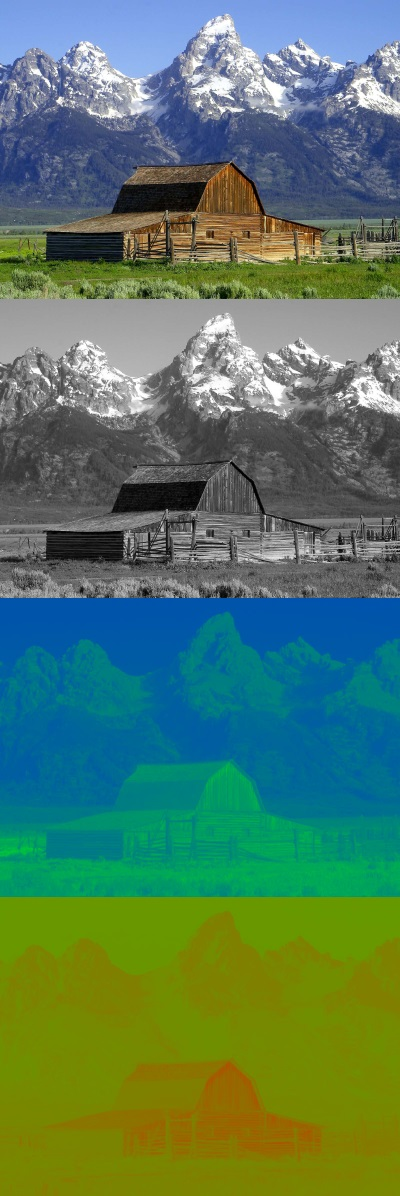
\includegraphics[totalheight=0.87\textheight,width=0.7\textwidth]{chapter2/yuv.jpg}
    \caption{Στην πρώτη εικόνα φαίνεται ένα καρέ με όλες τις συνιστώσες ενώ παρακάτω ξεχωριστά το YUV για το ίδιο καρέ \cite{wiki:yuv}.}
    \label{fig:yuv}
\end{figure}

\newpage
\section{Οργάνωση των pixels από τους κωδικοποιητές}
\label{section:sect23}

\indent Η πλειοψηφία των σημερινών κωδικοποιητών ομαδοποιούν τα pixels. Η πιο συνηθισμένη ομαδοποίηση είναι αυτή του macroblock, το κάθε καρέ διαιρείται σε μικρά πλακίδια σταθερής διάστασης NxN pixels οπού συνήθως N$=$16. Έτσι το καρέ του παραδείγματος μας αποτελείται από 518400/(16*16) $=$ 2025 macroblocks. Το κάθε macroblock μπορεί να σπάσει σε blocks και το κάθε block σε subblocks όπως φαίνεται στο Σχήμα~\ref{fig:mbpart}.

\begin{figure}[H]
  \centering
    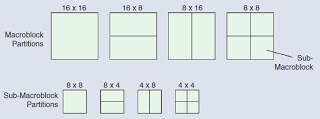
\includegraphics[width=0.7\textwidth]{chapter2/mbpart.jpg}
  \caption{Διαμερισμός του macroblock στον H.264.\cite{misc:mbpart}}
  \label{fig:mbpart}
\end{figure}

\indent Μέτα τον χωρισμό σε macroblocks οι κωδικοποιητές ομαδοποιούν τα καρέ σε Intra και Inter με τα τελευταία να χωρίζονται σε P και Β. Όλες οι παραπάνω κατηγοριοποιήσεις έχουν να κάνουν με τον μηχανισμό του Motion Estimation ο οποίος δημιουργεί διαφορές pixels (residuals). Κύριο χαρακτηριστικό των residuals είναι η μικρή τους ενέργεια (οι τίμες τους είναι κοντά στο 0).

\begin{itemize}
  \item Intra η αλλιώς I είναι τα καρέ που χρησιμοποιούν πληροφορία μόνο από το τρέχων καρέ για να βγάλουν τα residuals. Αυτό γίνετε απλά παίρνοντας τις τιμές των γειτονικών block και εφαρμόζοντας ένα mode π.χ μέσος όρος οπού το αποτέλεσμα αυτής αφαιρείται από τις τιμές των pixel του τρέχοντος block. Υπάρχουν διάφορα modes που μπορούν να γίνουν όπως φαίνεται και στο Σχήμα~\ref{fig:intrapred} και δοκιμάζονται κάθε φόρα όλα μέχρι να καταλήξουμε στο καλύτερο. Η απόδοση της συμπίεσης είναι η χειρότερη σε αυτήν την κατηγορία αλλά χωρίς αυτά το βίντεο δε θα μπορούσε να ξεκινήσει γιατί δεν θα είχαμε όλη την πληροφορία.

  \item P καρέ είναι αυτά τα οποία ψάχνουν το καλύτερο block για να κάνουν διαφορές από κάποιο αριθμό προηγούμενων καρέ όπως φαίνεται στο Σχήμα~\ref{fig:gop}

  \item Β καρέ είναι αυτά τα οποία ψάχνουν το καλύτερο block για να κάνουν διαφορές από κάποιο αριθμό προηγούμενων αλλά και επόμενων καρέ όπως φαίνεται στο Σχήμα~\ref{fig:gop}. Αυτά έχουν την καλύτερη απόδοση συμπίεσης αλλά η πολυπλοκότητα αποκωδικοποίησης είναι η μεγαλύτερη.
\end{itemize}

\indent Ένα επιπλέον στοιχείο των encoder είναι το group of pictures (GOP) το οποίο χαρακτηρίζει την σειρά με την οποία τα είδη των καρέ τοποθετούνται. Το GOP ξεκινάει από ένα I-frame συνεχίζει με P,B και περιοδικά έρχεται ένα Ι. Το GOP εξαρτάται από την εφαρμογή και μπορεί να έχει μεγάλες αποκλίσεις. Ένα τυπικό φαίνεται στο Σχήμα~\ref{fig:gop}

\indent Έτσι λοιπόν για να ανακατασκευαστεί ένα καρέ χρειάζεται την πληροφορία πρόβλεψης. Για τα Intra καρέ αυτή η πληροφορία είναι το mode που έγινε η κωδικοποίηση Σχήμα~\ref{fig:intrapred}. Για τα Inter είναι ένα διάνυσμα τριών διαστάσεων (motion vector) $mv = [ framenum , x , y]$ ,  οπού framenum είναι ο αριθμός του frame που βρίσκεται η πληροφορία και x,y οι συντεταγμένες του. Εννοείτε πως το framenum πρέπει ήδη να έχει αποκωδικοποιηθεί πλήρως είτε επειδή είναι Intra είτε επειδή έχει όλη την πληροφορία από προηγούμενα/επόμενα P,B καρέ.

\begin{figure}[H]
  \centering
    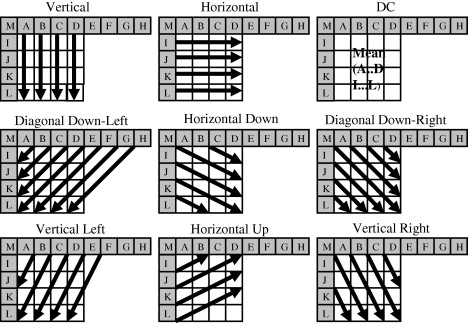
\includegraphics[width=0.7\textwidth]{chapter2/intrapred.jpg}
  \caption{Τρόποι που χρησιμοποιούνται στον Η.264 για Intra prediction. \cite{intrapred}}
    \label{fig:intrapred}
\end{figure}

\begin{figure}[H]
  \centering
    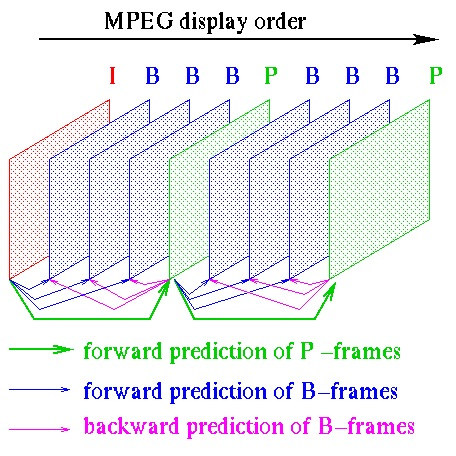
\includegraphics[width=0.7\textwidth]{chapter2/gop.jpg}
  \caption{Inter prediction στον mpeg και απεικόνιση ενός ενδεικτικοί GOP. \cite{misc:gop}}
  \label{fig:gop}
\end{figure}

\newpage

\section{Μετασχηματισμός}
\label{section:sect24}

\indent Έχοντας ο encoder κατασκευάσει τα residuals για το macroblock τότε το επόμενο βήμα είναι ένας μετασχηματισμός οπού συνήθως είναι ο DCT. Αυτό συμβαίνει γιατί ο μετασχηματισμός μας επιστρέφει πολλά 0 αν το σήμα μας είναι χαμηλής ενέργειας, όπως συμβαίνει με τα residuals. Έτσι χρησιμοποιώντας κάποιο ειδικό σύμβολο μπορούν να απεικονιστούν πολλά μηδενικά του μετασχηματισμού και να μειώσουμε το data rate μας όπως φαίνεται στο Σχήμα~\ref{eq:rle} μέσω της εφαρμογής του αλγορίθμου RLE (Run Length Encoding). Η σάρωση του macroblock δεν γίνετε γραμμικά αλλά με την μέθοδο του zigzag όπως στο Σχήμα~\ref{fig:zigzag} γιατί έτσι έχει παρατηρηθεί πως έχουμε παραπάνω μηδενικά στην σειρά άρα και καλύτερη απόδοση του RLE.
\\
\\
\begin{figure}[H]
\centering
$
\begin{array}{| c | c | c | c | c | c | c | c | c | c |}
    \hline 17 & 8 & 54 & 0 & 0 & 0 & 97 & 5 & 0 & 16 \\ \hline
\end{array}
\xrightarrow[RLE]{}
\begin{array}{| c | c | c | c | c | c | c | c |}
    \hline 17 & 8 & 54 & [0,3]  & 97 & 5 & [0,2] & 16 \\ \hline
\end{array}
$
\caption{Παραδείγμα χρήσης RLE}
\label{eq:rle}
\end{figure}

\begin{figure}[H]
  \centering
  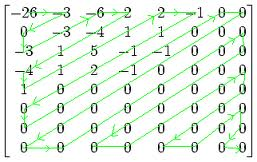
\includegraphics[width=0.7\textwidth]{chapter2/zigzag.jpg}
  \caption{Σάρωση ZigZag. \cite{misc:zigzag}}
  \label{fig:zigzag}
\end{figure}

\newpage
\section{Κβαντοποίηση}
\label{section:sect25}

\indent Η κβαντοποίηση είναι το σημείο που σε κάθε encoder εισάγεται ο θόρυβος, θα μπορούσε να θεωρηθεί και ο DCT,iDCT λόγο ακρίβειας αλλά εκεί το σφάλμα είναι παρά πολύ μικρό. Μετά τον μετασχηματισμό τα residuals έχουν αντικατασταθεί με συντελεστές οι οποίοι είναι πραγματικοί αριθμό. Η τακτική που εφαρμόζεται είναι να γίνει ακέραια διαίρεση ο συντελεστής της κάθε συχνότητας με έναν σταθερό αριθμό διαφορετικό για κάθε συχνότητα Πίνακας~\ref{table:quanttable}. Επομένως για τον δεδομένο πίνακα κβαντοποίησης με τους συντελεστές του Πίνακα~\ref{table:coeff} έχουμε τα αποτελέσματα στον Πίνακα~\ref{table:results} τα οποία είναι αυτά που θα δοθούν σε κάποιον entropy encoder για να συμπιεστούν.

\indent Ο Πίνακας~\ref{table:quanttable} μεταβάλετε με βάση μια μεταβλητή που καθορίζει την ποιότητα του βίντεο. Στον H.264 το $QP \in [0,51] $. Στο 0 δεν γίνετε καθόλου κβαντοποίηση και όσο το QP αυξάνει τόσο η ποιότητα πέφτει. Αυτό συμβαίνει γιατί το QP πολλαπλασιάζεται με τον Πίνακα~\ref{table:quanttable} και οι τιμές του μεγαλώνουν. Επομένως στην ακέραια διαίρεση χάνουμε περισσότερο πληροφορία διότι διαιρούμε με μεγαλύτερο αριθμό. Κερδίζουμε όμως σε μέγεθος γιατί έτσι προκύπτουν περισσότερα μηδενικά.

\begin{table}[H]
    \begin{center}
        \begin{tabular}{| c  c  c  c  c  c  c  c |}
        \hline
        16 & 11 & 10 & 16 & 24 & 40 & 51 & 61 \\
        12 & 12 & 14 & 19 & 26 & 58 & 60 & 55 \\
        14 & 14 & 16 & 24 & 40 & 57 & 69 & 56 \\
        14 & 17 & 22 & 29 & 51 & 87 & 80 & 62 \\
        18 & 22 & 37 & 56 & 68 & 109 & 103 & 77 \\
        24 & 35 & 55 & 64 & 81 & 104 & 113 & 92 \\
        49 & 64 & 78 & 87 & 103 & 121 & 120 & 101 \\
        72 & 92 & 95 & 98 & 112 & 100 & 103 & 99 \\
        \hline
        \end{tabular}
    \end{center}
    \caption{Πίνακας Κβαντοποίησης. \cite{wiki:jpeg}}
    \label{table:quanttable}
\end{table}

\begin{table}[H]
    \begin{center}
        \begin{tabular}{| c  c  c  c  c  c  c  c |}
        \hline
        -415.38 & -30.19 & -61.20 & 27.24 & 56.13 & -20.10 & -2.39 & 0.46 \\
        4.47 & -21.86 & -60.76 & 10.25 & 13.15 & -7.09 & -8.54 & 4.88 \\
        -46.83 & 7.37 & 77.13 & -24.56 & -28.91 & 9.93 & 5.42 & -5.65 \\
        -48.53 & 12.07 & 34.10 & -14.76 & -10.24 & 6.30 & 1.83 & 1.95 \\
        12.12 & -6.55 & -13.20 & -3.95 & -1.88 & 1.75 & -2.79 & 3.14 \\
        -7.73 & 2.91 & 2.38 & -5.94 & -2.38 & 0.94 & 4.30 & 1.84 \\
        -1.03 & 0.18 & 0.42 & -2.42 & -0.88 & -3.02 & 4.12 & -0.66 \\
        -0.17 & 0.14 & -1.07 & -4.19 & -1.17 & -0.10 & 0.70 & 1.68 \\
        \hline
        \end{tabular}
    \end{center}
    \caption{Παράδειγμα συντελεστών DCT 8x8. \cite{wiki:jpeg}}
    \label{table:coeff}
\end{table}

\begin{table}[H]
    \begin{center}
        \begin{tabular}{| c  c  c  c  c  c  c  c |}
        \hline
        -26 & -3 & -6 & 2 & 2 & -1 & 0 & 0 \\
        0 & -2 & -4 & 1 & 1 & 0 & 0 & 0 \\
        -3 & 1 & 5 & -1 & -1 & 0 & 0 & 0 \\
        -3 & 1 & 2 & -1 & 0 & 0 & 0 & 0 \\
         1 & 0 & 0 & 0 & 0 & 0 & 0 & 0 \\
        0 & 0 & 0 & 0 & 0 & 0 & 0 & 0 \\
        0 & 0 & 0 & 0 & 0 & 0 & 0 & 0 \\
        0 & 0 & 0 & 0 & 0 & 0 & 0 & 0 \\
        \hline
        \end{tabular}
    \end{center}
    \caption{Κβαντοποιημένοι συντελεστές DCT. \cite{wiki:jpeg}}
    \label{table:results}
\end{table}

\section{Αποκωδικοποίηση βίντεο}
\label{section:sect26}

\indent Για την αποκωδικοποίηση κάνουμε όλα τα βήματα που κάνει ο encoder με την ανάποδη σειρά.

\begin{itemize}
  \item Μετά την entropy decoding τα νούμερα πολλαπλασιάζονται με τα στοιχεία του πίνακα κβαντοποίησης. Έτσι ανακτούνται οι συντελεστές του μετασχηματισμού με έχοντας πλέον εισαχθεί το σφάλμα που προέκυψε λόγο της ακέραιας διαίρεσης.
  \item Γίνετε αντίστροφος μετασχηματισμός και ανακτούνται τα residuals.
  \item Τέλος το Motion Decomposition βρίσκει τα δύο block που χρησιμοποιήθηκαν για να παραχθούν τα residuals (μέσω των motion vectors) και τα προσθέτουμε για να πάρουμε τα ανακατασκευασμένα pixels.
\end{itemize}

\section{Ποιότητα Βίντεο}
\label{section:sect27}

\indent Με τον όρο ποιότητα βίντεο ορίζουμε τον μέσω όρο του άθροισματος των διαφόρων στο τετράγωνο MSE (Mean Square Error) όλων τον pixels μεταξύ του ασυμπίεστου βίντεο και του αυτού που αποσυμπιέσαμε. \begin{equation}
\text{MSE} =
\frac{\displaystyle\sum_{i=1}^{X*Y}
(Source_{pixel_i}-Reconstructed_{pixel_i})^{2}}{X*Y}
\end{equation}

\indent Συνήθως το μετατρέπουμε σε PSNR με μονάδα μέτρησης το \si{}{dB} με τον τύπο  $ PSNR = 10*\log_{10}{\frac{MAX_i^2}{MSE}}$ οπού το $MAX_i$ είναι η μέγιστη τιμή που μπορεί να πάρει ένα pixel. Αυτό εξαρτάται από το bitdepth, π.χ αν έχουμε bitdepth=8bits τότε $ MAX_i=255$.

\indent Ο μέσος όρος του PSNR όλων των καρέ μας δίνει την ποιότητα του βίντεο.

\section{Δομή του Η.264}
\label{section:sect28}

\indent Παρακάτω βλέπουμε την δομή του H.264 encoder Σχήμα~\ref{fig:h264}. Το σημείο με το γκρι είναι το κομμάτι του decoder. Κάθε encoder υλοποιεί στο εσωτερικό του και έναν decoder αλλά σε αυτή την διπλωματική δεν θα εξηγήσουμε κάτι παραπάνω γιατί δεν βοηθάει στην κατανόηση της.

\begin{figure}[h]
    \centering
    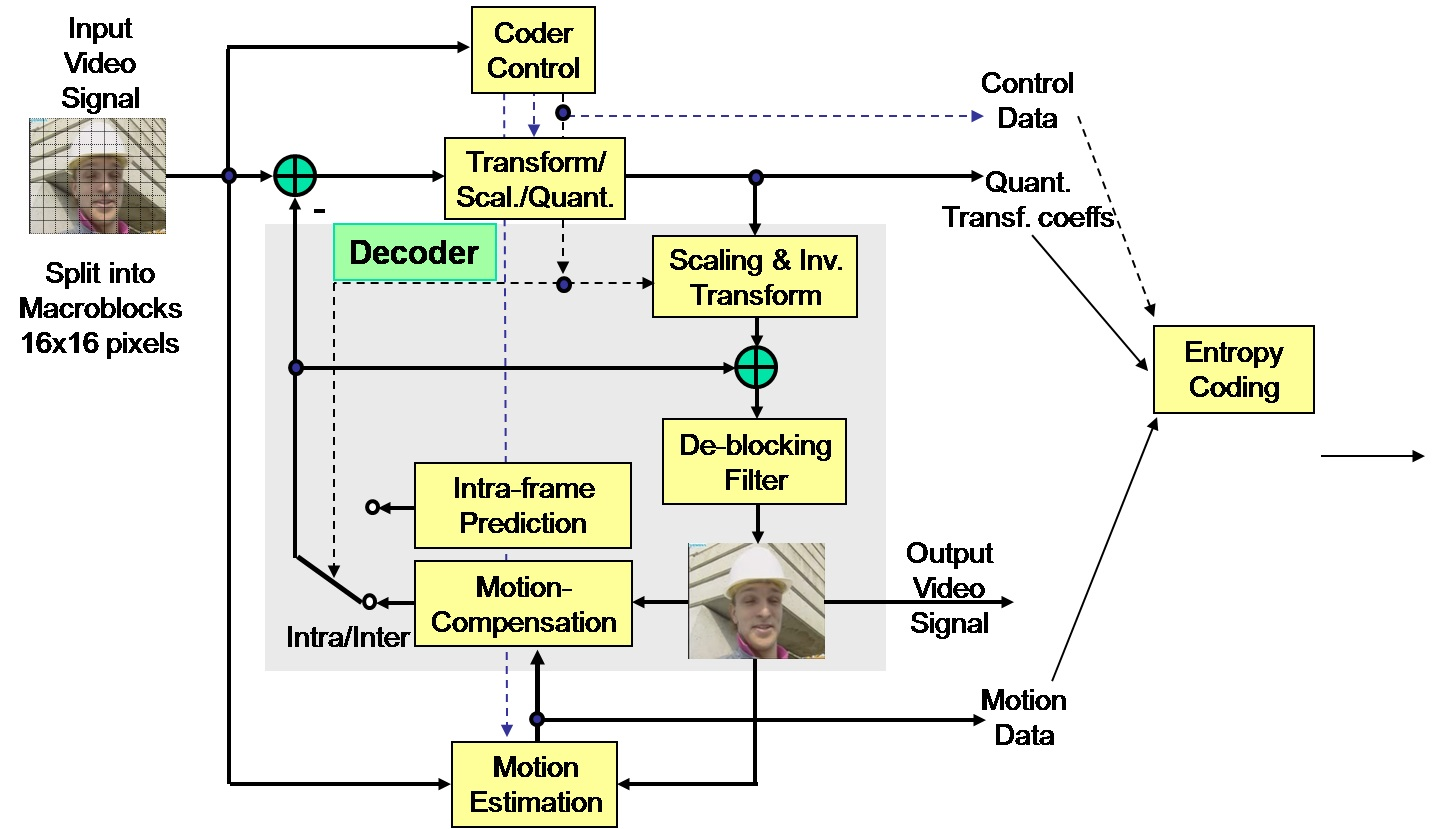
\includegraphics[width=0.7\textwidth]{chapter2/h264.jpg}
    \caption{H.264 encoder structure. \cite{misc:structure}}
    \label{fig:h264}
\end{figure}
